%!TEX program = lualatex
% ============================================================================
% BEAMER PRESENTATION - MAIN FILE
% ============================================================================
% Compile: lualatex 00_main.tex (preferred) or pdflatex 00_main.tex (fallback)
%
% FILE STRUCTURE:
%   00_main.tex       - This file (presentation info + includes)
%   00_template.tex   - Template settings (modify for theme changes)
%   01_slides.tex     - Your content slides
%   99_bibliography.tex - References
%
% ============================================================================
% RULES TO FOLLOW
% ============================================================================
%
% LABELS: fig:name, tab:name, eq:name, sec:name
% CHARS:  ASCII only, escape \% \& \$ \# \_ \{ \}
% MATH:   Use align/multline for long equations
% CITE:   Space before \cite: "shown in \cite{}" not "in\cite{}"
%
% ============================================================================
% PRESENTATION INFO
% ============================================================================

\newcommand{\AuthorName}{Basem Rajjoub}
\newcommand{\AuthorAffiliation}{IWES, LUH}
\newcommand{\PresentationTitle}{Presentation Title}
\newcommand{\PresentationSubtitle}{Optional Subtitle}
\newcommand{\PresentationDate}{May 19, 2026}

% ============================================================================
% LOAD TEMPLATE
% ============================================================================

%!TEX root = 00_main.tex
%!TEX program = lualatex
% ============================================================================
% BEAMER TEMPLATE - DO NOT MODIFY
% ============================================================================
% This file contains all template logic, packages, and theme configuration.
% Only modify 00_main.tex for presentation content.
%
% COMPILER: LuaLaTeX (preferred), XeLaTeX, or pdfLaTeX (fallback fonts)
% ============================================================================

% ============================================================================
% DEFAULT TEMPLATE SETTINGS (rarely need to change)
% ============================================================================

% --- Logo Settings ---
\newcommand{\LogoLeftFile}{02-IWES-Logo.pdf}
\newcommand{\LogoRightFile}{01-LUH-Logo.pdf}
\newcommand{\LogoHeight}{0.5cm}
\newcommand{\TitleLogoHeight}{1.2cm}

% --- Title Page Background Image ---
\newcommand{\TitleBackgroundImage}{background.png}
\newcommand{\TitleBackgroundHeight}{0.5\paperheight}

% --- Colors (RGB values, 0-1 scale) ---
\newcommand{\MainBlueR}{0.090}              % 23/255
\newcommand{\MainBlueG}{0.318}              % 81/255
\newcommand{\MainBlueB}{0.616}              % 157/255
\newcommand{\FooterGrayR}{0.8}
\newcommand{\FooterGrayG}{0.8}
\newcommand{\FooterGrayB}{0.8}
\newcommand{\FooterAccentR}{0.6}
\newcommand{\FooterAccentG}{0.8}
\newcommand{\FooterAccentB}{0.2}

% --- Footer Settings ---
\newcommand{\FooterBarHeight}{0.5cm}
\newcommand{\FooterAccentWidth}{1cm}
\newcommand{\FooterAccentHeight}{0.1cm}

% --- Frame Content Margins/Padding ---
\newcommand{\FrameMarginLeft}{1cm}
\newcommand{\FrameMarginRight}{1cm}
\newcommand{\FrameTopPadding}{0.5cm}
\newcommand{\FrameBottomPadding}{0.5cm}

% --- Font Size Settings ---
\newcommand{\BaseFontSize}{11pt}
\newcommand{\TitleFontSize}{\Huge}
\newcommand{\SubtitleFontSize}{\large}
\newcommand{\AuthorFontSize}{\large}
\newcommand{\DateFontSize}{\normalsize}
\newcommand{\FrameTitleSize}{\large}
\newcommand{\FooterFontSize}{\tiny}

% --- Font Settings (XeLaTeX) ---
% Main font options: "Rotis Sans Serif Std", "Arial", "Helvetica Neue", etc.
\newcommand{\MainFont}{Rotis Sans Serif Std}
\newcommand{\MonoFont}{Consolas}    % For code listings

% ============================================================================
% DOCUMENT CLASS
% ============================================================================

\documentclass[aspectratio=169, \BaseFontSize]{beamer}

% ============================================================================
% PACKAGES
% ============================================================================

% Note: With XeLaTeX, we don't need inputenc/fontenc
\usepackage{graphicx}
\usepackage{amsmath}
\usepackage{amssymb}
\usepackage{tikz}
\usepackage{xcolor}
\usepackage{booktabs}
\usepackage{hyperref}               % Links (internal and external)
\usepackage{attachfile2}            % Embed files in PDF
\usepackage{listings}               % Code listings
\usepackage{multimedia}             % Video embedding
\usepackage{qrcode}                 % QR code generation
\usepackage{pgfgantt}               % Gantt charts

% --- Font Configuration ---
% Detects compiler and uses appropriate font setup:
%   - LuaLaTeX/XeLaTeX: fontspec with Rotis (falls back to TeX Gyre Heros if missing)
%   - pdfLaTeX: TeX Gyre Heros (Helvetica clone)

\usepackage{iftex}  % Provides \ifluatex, \ifxetex, \ifpdftex

\ifluatex
    % LuaLaTeX configuration
    \usepackage{fontspec}
    \IfFileExists{./Rotis/RotisSansSerifStd-Regular.otf}{%
        % Rotis font found - use it
        \setsansfont{RotisSansSerifStd}[
            Path = ./Rotis/,
            Extension = .otf,
            UprightFont = *-Regular,
            BoldFont = *-Bold,
            ItalicFont = *-Italic,
            BoldItalicFont = *-Bold,
        ]
    }{%
        % Rotis not found - use TeX Gyre Heros (Helvetica clone)
        \setsansfont{TeX Gyre Heros}
    }
    \setmonofont{Consolas}[Scale=0.9]
\else\ifxetex
    % XeLaTeX configuration
    \usepackage{fontspec}
    \IfFileExists{./Rotis/RotisSansSerifStd-Regular.otf}{%
        \setsansfont{RotisSansSerifStd}[
            Path = ./Rotis/,
            Extension = .otf,
            UprightFont = *-Regular,
            BoldFont = *-Bold,
            ItalicFont = *-Italic,
            BoldItalicFont = *-Bold,
        ]
    }{%
        \setsansfont{TeX Gyre Heros}
    }
    \setmonofont{Consolas}[Scale=0.9]
\else
    % pdfLaTeX configuration - use standard packages
    \usepackage[T1]{fontenc}
    \usepackage{tgheros}        % TeX Gyre Heros (Helvetica clone)
    \usepackage[scaled=0.9]{beramono}  % Bera Mono for code
\fi\fi

\renewcommand{\familydefault}{\sfdefault}

% ============================================================================
% COLOR DEFINITIONS
% ============================================================================

\definecolor{mainblue}{rgb}{\MainBlueR,\MainBlueG,\MainBlueB}
\definecolor{footergray}{rgb}{\FooterGrayR,\FooterGrayG,\FooterGrayB}
\definecolor{footeraccent}{rgb}{\FooterAccentR,\FooterAccentG,\FooterAccentB}

% Configure hyperlinks
\hypersetup{
    colorlinks=true,
    linkcolor=mainblue,
    urlcolor=mainblue,
    citecolor=mainblue
}

% --- Code Listings Configuration ---
\lstdefinestyle{default}{
    basicstyle=\ttfamily\scriptsize,
    keywordstyle=\color{mainblue}\bfseries,
    commentstyle=\color{gray}\itshape,
    stringstyle=\color{red!70!black},
    numberstyle=\tiny\color{gray},
    numbers=left,
    numbersep=5pt,
    frame=single,
    framerule=0.5pt,
    rulecolor=\color{gray},
    backgroundcolor=\color{gray!5},
    breaklines=true,
    breakatwhitespace=true,
    tabsize=4,
    showstringspaces=false,
    captionpos=b
}
\lstdefinestyle{terminal}{
    basicstyle=\ttfamily\scriptsize\color{white},
    backgroundcolor=\color{black!90},
    frame=single,
    framerule=0pt,
    numbers=none,
    breaklines=true
}
\lstset{style=default}

% ============================================================================
% BEAMER THEME CONFIGURATION
% ============================================================================

\usetheme{default}
\usecolortheme{default}

% Remove navigation symbols
\setbeamertemplate{navigation symbols}{}

% Set colors
\setbeamercolor{title}{fg=mainblue}
\setbeamercolor{frametitle}{fg=mainblue}
\setbeamercolor{structure}{fg=mainblue}
\setbeamercolor{itemize item}{fg=mainblue}
\setbeamercolor{itemize subitem}{fg=mainblue}
\setbeamercolor{enumerate item}{fg=mainblue}
\setbeamercolor{enumerate subitem}{fg=mainblue}

% Background
\setbeamercolor{background canvas}{bg=white}

% Bullet styles
\setbeamertemplate{itemize item}{\textbullet}
\setbeamertemplate{itemize subitem}{--}
\setbeamertemplate{enumerate items}[default]

% Frame content margins
\setbeamersize{
    text margin left=\FrameMarginLeft,
    text margin right=\FrameMarginRight
}

% ============================================================================
% CUSTOM HEADER (HEADLINE) WITH LOGOS
% ============================================================================

\setbeamertemplate{headline}{%
    \begin{tikzpicture}[remember picture, overlay]
        % Left logo
        \node[anchor=north west, inner sep=0.3cm] at (current page.north west) {%
            \includegraphics[height=\LogoHeight]{\LogoLeftFile}%
        };
        % Right logo
        \node[anchor=north east, inner sep=0.3cm] at (current page.north east) {%
            \includegraphics[height=\LogoHeight]{\LogoRightFile}%
        };
    \end{tikzpicture}%
    \vspace{\FrameTopPadding}%
}

% ============================================================================
% CUSTOM FOOTER (FOOTLINE) WITH GRAY BAR AND ACCENT
% ============================================================================

\setbeamertemplate{footline}{%
    \vspace{\FrameBottomPadding}%
    \begin{tikzpicture}[remember picture, overlay]
        % Gray bar background
        \fill[footergray] (current page.south west) rectangle
            ([yshift=\FooterBarHeight]current page.south east);
        % Author name and date (left)
        \node[anchor=south west, inner sep=0.15cm, text=black, font=\FooterFontSize]
            at (current page.south west) {%
                \AuthorName{} \textbar{} \PresentationDate%
            };
        % Page number (right)
        \node[anchor=south east, inner sep=0.15cm, text=black, font=\FooterFontSize]
            at ([xshift=-0.5cm]current page.south east) {%
                \insertframenumber{}/\inserttotalframenumber%
            };
        % Accent rectangle (aligned with right logo)
        \fill[footeraccent] ([xshift=-0.3cm-\FooterAccentWidth, yshift=\FooterBarHeight]current page.south east) rectangle
            ([xshift=-0.3cm, yshift=\FooterBarHeight-\FooterAccentHeight]current page.south east);
    \end{tikzpicture}%
}

% ============================================================================
% FRAME TITLE FORMATTING
% ============================================================================

\setbeamertemplate{frametitle}{%
    \vspace{0.5cm}%
    {\FrameTitleSize\textbf{\insertframetitle}}%
    \par%
}

% ============================================================================
% TITLE PAGE TEMPLATE
% ============================================================================

\defbeamertemplate*{title page}{customtitle}[1][]{%
    \begin{tikzpicture}[remember picture, overlay]
        % Left logo (bigger on title page)
        \node[anchor=north west, inner sep=0.3cm] at (current page.north west) {%
            \includegraphics[height=\TitleLogoHeight]{\LogoLeftFile}%
        };
        % Right logo (bigger on title page)
        \node[anchor=north east, inner sep=0.3cm] at (current page.north east) {%
            \includegraphics[height=\TitleLogoHeight]{\LogoRightFile}%
        };
        % Background image at bottom
        \node[anchor=south, inner sep=0] at (current page.south) {%
            \includegraphics[width=\paperwidth, height=\TitleBackgroundHeight, keepaspectratio=false]{\TitleBackgroundImage}%
        };
        % Date anchored to bottom right corner
        \node[anchor=south east, inner sep=0.5cm] at (current page.south east) {%
            \DateFontSize\PresentationDate%
        };
    \end{tikzpicture}%
    % \vfill
    % \begin{center}
        {\TitleFontSize\bfseries\color{mainblue}\PresentationTitle\par}
        \vspace{0.5cm}
        % {\SubtitleFontSize\color{gray}\PresentationSubtitle\par}
        % \vspace{1cm}
        {\AuthorFontSize\AuthorName \hspace{1cm} \normalsize\AuthorAffiliation\par}
    % \end{center}
    \vfill
}

% ============================================================================
% DOCUMENT INFO
% ============================================================================

\title{\PresentationTitle}
\author{\AuthorName}
\date{\PresentationDate}


% ============================================================================
% DOCUMENT
% ============================================================================

\begin{document}

% --- Title Slide ---
\begin{frame}[plain]
    \titlepage
\end{frame}

% --- Outline ---
\begin{frame}{Outline}
    \tableofcontents
\end{frame}

% ============================================================================
% SLIDES
% ============================================================================

%!TEX root = 00_main.tex
% ============================================================================
% CONTENT SLIDES
% ============================================================================
% Add your presentation content here.
% Create additional files (02_slides.tex, etc.) for more sections.
% ============================================================================

\section{Introduction}

% --- Motivation Slide ---
\begin{frame}{Wind Energy: Global Context}
    \begin{itemize}
        \item Wind power capacity exceeded 900 GW globally in 2023
        \item Offshore wind growing at 25\% annually
            \begin{itemize}
                \item Floating foundations enable deeper water installations
                \item Larger rotors (15+ MW turbines) improve capacity factors
            \end{itemize}
        \item Key engineering challenges:
            \begin{itemize}
                \item Fatigue life prediction under stochastic loading
                \item Aeroelastic stability of flexible blades
            \end{itemize}
        \item Cost reduction target: below 50 EUR/MWh by 2030
    \end{itemize}
\end{frame}

\section{Theory}

% --- Aerodynamics Slide ---
\begin{frame}{Wind Turbine Aerodynamics}
    The power extracted by a wind turbine is given by:
    \begin{equation}
        P = \frac{1}{2} \rho A C_p v^3
        \label{eq:power}
    \end{equation}
    where $\rho$ is air density, $A$ is rotor area, and $v$ is wind speed.

    \vspace{0.3cm}

    The Betz limit defines the maximum power coefficient:
    \begin{align}
        C_{p,\text{max}} &= \frac{16}{27} \approx 0.593 \label{eq:betz}\\
        a_{\text{opt}} &= \frac{1}{3} \label{eq:induction}
    \end{align}

    \vspace{0.3cm}

    Modern turbines achieve $C_p \approx 0.45$ (see Equation~\eqref{eq:betz}).
\end{frame}

\section{Results}

% --- Single Figure Slide ---
\begin{frame}{Power Curve Comparison}
    \begin{center}
        
\includegraphics[height=4cm]{example_figure.png}
    \end{center}
    \begin{center}
        \textbf{Figure 1:} Measured vs. simulated power curve for a 5 MW offshore turbine.
    \end{center}
\end{frame}

% --- Two Figures Side-by-Side Slide ---
\begin{frame}{Blade Load Distribution}
    \begin{columns}[T]
        \begin{column}{0.4\textwidth}
            \centering
            
\includegraphics[width=\textwidth]{example_figure.png}

            \textbf{(a)} Flapwise bending moment
        \end{column}
        \begin{column}{0.4\textwidth}
            \centering
            
\includegraphics[width=\textwidth]{example_figure.png}

            \textbf{(b)} Edgewise bending moment
        \end{column}
    \end{columns}
\end{frame}

% --- Figure with Bullet Points Slide ---
\begin{frame}{Fatigue Damage Analysis}
    \begin{columns}[T]
        \begin{column}{0.45\textwidth}
            \begin{itemize}
                \item Rainflow counting applied to load time series
                \item Damage equivalent load (DEL): 12.5 MNm
                \item Critical location: blade root transition
                \item Safety factor of 1.35 applied per IEC 61400-1
                \item 20-year design life validated
            \end{itemize}
        \end{column}
        \begin{column}{0.45\textwidth}
            \centering
            
\includegraphics[width=\textwidth]{example_figure.png}

            {\small\textbf{Figure:} S-N curve with Goodman correction}
        \end{column}
    \end{columns}
\end{frame}

\section{Conclusion}

% --- Summary Slide ---
\begin{frame}{Summary and Outlook}
    \begin{enumerate}
        \item Aeroelastic model validated against field measurements
        \item Fatigue life meets 20-year design requirements
        \item Blade pitch control reduces extreme loads by 15\%
        \item Future work: investigate wake effects in wind farm layout
    \end{enumerate}

    \vspace{0.5cm}

    \textbf{Thank you for your attention!}

    \vspace{0.3cm}

    Questions?
\end{frame}

% %!TEX root = 00_main.tex
% ============================================================================
% ADVANCED SLIDES - DIAGRAMS, EMBEDS, AND SPECIAL FEATURES
% ============================================================================

\section{Diagrams and Drawings}

% --- TikZ Flowchart ---
\begin{frame}{Process Flowchart (TikZ)}
    \centering
    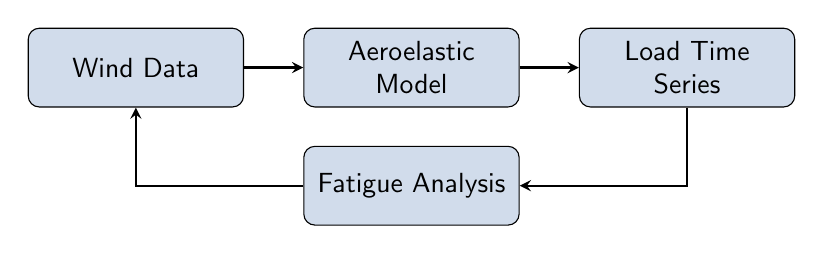
\begin{tikzpicture}[node distance=1.5cm, auto,
        block/.style={rectangle, draw, fill=mainblue!20, text width=2.5cm, text centered, rounded corners, minimum height=1cm},
        arrow/.style={->, >=stealth, thick}]

        \node[block] (input) {Wind Data};
        \node[block, right of=input, xshift=2cm] (process) {Aeroelastic Model};
        \node[block, right of=process, xshift=2cm] (output) {Load Time Series};
        \node[block, below of=process] (fatigue) {Fatigue Analysis};

        \draw[arrow] (input) -- (process);
        \draw[arrow] (process) -- (output);
        \draw[arrow] (output) |- (fatigue);
        \draw[arrow] (fatigue) -| (input);
    \end{tikzpicture}

    \vspace{0.5cm}
    {\small Simulation workflow for wind turbine design certification.}
\end{frame}

% --- TikZ Plot ---
\begin{frame}{Data Plot (TikZ)}
    \centering
    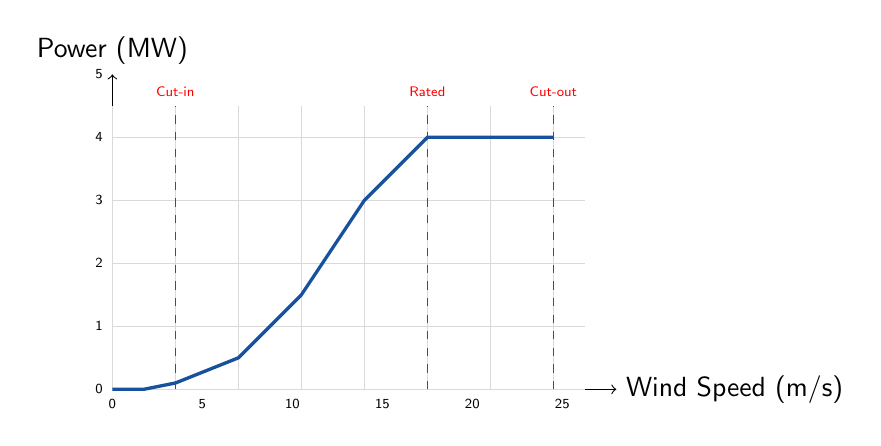
\begin{tikzpicture}[scale=0.8]
        \draw[->] (0,0) -- (8,0) node[right] {Wind Speed (m/s)};
        \draw[->] (0,0) -- (0,5) node[above] {Power (MW)};

        % Grid
        \draw[gray!30] (0,0) grid (7.5,4.5);

        % Power curve
        \draw[mainblue, very thick]
            (0,0) -- (0.5,0) -- (1,0.1) -- (2,0.5) -- (3,1.5) -- (4,3) -- (5,4) -- (6,4) -- (7,4);

        % Labels
        \foreach \x in {0,5,10,15,20,25} {
            \node[below, font=\tiny] at (\x/3.5,0) {\x};
        }
        \foreach \y in {0,1,2,3,4,5} {
            \node[left, font=\tiny] at (0,\y) {\y};
        }

        % Annotations
        \draw[red, dashed] (1,0) -- (1,4.5) node[above, font=\tiny] {Cut-in};
        \draw[red, dashed] (5,0) -- (5,4.5) node[above, font=\tiny] {Rated};
        \draw[red, dashed] (7,0) -- (7,4.5) node[above, font=\tiny] {Cut-out};
    \end{tikzpicture}

    \vspace{0.3cm}
    {\small Typical power curve of a 5 MW wind turbine.}
\end{frame}

% --- TikZ Block Diagram ---
\begin{frame}{Control System Block Diagram}
    \centering
    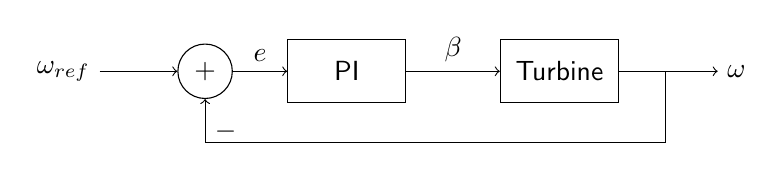
\begin{tikzpicture}[scale=0.9,
        block/.style={rectangle, draw, minimum height=0.8cm, minimum width=1.5cm},
        sum/.style={circle, draw, minimum size=0.5cm}]

        \node[sum] (sum) at (0,0) {$+$};
        \node[block] (controller) at (2,0) {PI};
        \node[block] (plant) at (5,0) {Turbine};
        \node (output) at (7.5,0) {$\omega$};
        \node (input) at (-2,0) {$\omega_{ref}$};

        \draw[->] (input) -- (sum);
        \draw[->] (sum) -- (controller) node[midway, above] {$e$};
        \draw[->] (controller) -- (plant) node[midway, above] {$\beta$};
        \draw[->] (plant) -- (output);
        \draw[->] (6.5,0) -- (6.5,-1) -- (0,-1) -- (sum) node[near start, right] {$-$};
    \end{tikzpicture}

    \vspace{0.5cm}
    {\small Pitch control loop for rotor speed regulation.}
\end{frame}

\section{External Links and Embedded Files}

% --- Links to External Files ---
\begin{frame}{Links to External Files}
    Click links below to open files (must be in same folder as PDF):

    \vspace{0.5cm}

    \begin{itemize}
        \item \href{run:example_figure.png}{Open example\_figure.png} (external link)
        \item \href{run:00_main.tex}{Open source file (00\_main.tex)}
        \item \href{run:01_slides.tex}{Open slides source}
    \end{itemize}

    \vspace{0.5cm}

    Web links:
    \begin{itemize}
        \item \href{https://www.nrel.gov/wind/}{NREL Wind Energy Research}
        \item \href{https://www.iec.ch}{IEC Standards}
    \end{itemize}

    \vspace{0.3cm}
    {\small\textit{Note: External file links work when PDF is in the same folder.}}
\end{frame}

% --- Embedded/Attached Files ---
\begin{frame}[fragile]{Embedded Files in PDF}
    Files can be attached to this PDF using attachfile2 package:

    \vspace{0.3cm}

    \begin{lstlisting}[basicstyle=\ttfamily\small, frame=none, numbers=none]
\textattachfile{data.csv}{Click to open data}
\textattachfile{code.py}{Click to open code}
    \end{lstlisting}

    \vspace{0.3cm}

    {\small Files are embedded inside the PDF and can be extracted by the viewer.}

    \vspace{0.3cm}

    \textit{Useful for sharing data, code, or supplementary materials.}

    \vspace{0.3cm}

    {\footnotesize\textbf{Note:} Uncomment attachfile2 examples when files exist.}
\end{frame}

\section{Beamer Special Features}

% --- Overlays/Animations ---
\begin{frame}{Step-by-Step Reveal (Overlays)}
    Design process phases:

    \begin{enumerate}
        \item<1-> \textbf{Conceptual Design} -- Define requirements
        \item<2-> \textbf{Preliminary Design} -- Initial sizing
        \item<3-> \textbf{Detailed Design} -- FEM analysis
        \item<4-> \textbf{Validation} -- Testing and certification
    \end{enumerate}

    \vspace{0.5cm}

    \only<1>{Start with project requirements and constraints.}
    \only<2>{Perform initial aerodynamic and structural sizing.}
    \only<3>{Run detailed simulations and optimize.}
    \only<4>{Validate against standards (IEC 61400).}
\end{frame}

% --- Blocks ---
\begin{frame}{Information Blocks}
    \begin{block}{Definition}
        The \textbf{capacity factor} is the ratio of actual energy produced to the maximum possible energy output over a period.
    \end{block}

    \begin{exampleblock}{Example}
        A 5 MW turbine producing 15,000 MWh/year has a capacity factor of:
        $CF = \frac{15000}{5 \times 8760} = 34.2\%$
    \end{exampleblock}

    \begin{alertblock}{Warning}
        Capacity factor varies significantly with site conditions and turbine selection.
    \end{alertblock}
\end{frame}

% --- Table Example ---
\begin{frame}{Data Table}
    \centering
    \begin{tabular}{lrrr}
        \toprule
        \textbf{Parameter} & \textbf{IEA 15 MW} & \textbf{DTU 10 MW} & \textbf{NREL 5 MW} \\
        \midrule
        Rated Power (MW)    & 15.0  & 10.0  & 5.0   \\
        Rotor Diameter (m)  & 240   & 178   & 126   \\
        Hub Height (m)      & 150   & 119   & 90    \\
        Tip Speed (m/s)     & 95    & 90    & 80    \\
        \bottomrule
    \end{tabular}

    \vspace{0.5cm}
    {\small Reference wind turbine specifications for research.}
\end{frame}

% --- Multi-column with Pause ---
\begin{frame}{Comparison Layout}
    \begin{columns}[T]
        \begin{column}{0.48\textwidth}
            \textbf{Onshore Wind}
            \begin{itemize}
                \item Lower installation cost
                \item Easier maintenance access
                \item Visual/noise concerns
                \item Limited to smaller turbines
            \end{itemize}
        \end{column}
        \begin{column}{0.48\textwidth}
            \textbf{Offshore Wind}
            \begin{itemize}
                \item Higher wind speeds
                \item Larger turbines possible
                \item Higher CAPEX/OPEX
                \item Complex logistics
            \end{itemize}
        \end{column}
    \end{columns}
\end{frame}

% %!TEX root = 00_main.tex
% ============================================================================
% ADVANCED SLIDES - CODE, VIDEOS, QR CODES, GANTT CHARTS
% ============================================================================

\section{Code Listings}

% --- Python Code ---
\begin{frame}[fragile]{Python Code Example}
    \begin{lstlisting}[language=Python, caption={Wind power calculation}]
import numpy as np

def wind_power(rho, A, Cp, v):
    """Calculate wind turbine power output.

    Args:
        rho: Air density (kg/m^3)
        A: Rotor area (m^2)
        Cp: Power coefficient
        v: Wind speed (m/s)
    """
    return 0.5 * rho * A * Cp * v**3

# Example: 5 MW turbine
P = wind_power(1.225, 12469, 0.45, 12)
print(f"Power: {P/1e6:.2f} MW")
    \end{lstlisting}
\end{frame}

% --- MATLAB Code ---
\begin{frame}[fragile]{MATLAB Code Example}
    \begin{lstlisting}[language=Matlab, caption={Blade element momentum theory}]
function [a, ap] = bem_iteration(lambda, theta, Cl, Cd)
    % BEM iteration for axial and tangential induction
    sigma = 0.05;  % Solidity
    phi = atan(1 / lambda);

    % Thrust and torque coefficients
    Ct = sigma * (Cl*cos(phi) + Cd*sin(phi));
    Cq = sigma * (Cl*sin(phi) - Cd*cos(phi));

    % Induction factors
    a = 1 / (1 + 4*sin(phi)^2 / (sigma*Cl*cos(phi)));
    ap = 1 / (4*cos(phi) / (sigma*Cl) - 1);
end
    \end{lstlisting}
\end{frame}

% --- Inline Code ---
\begin{frame}[fragile]{Code Snippets and Terminal Output}
    \textbf{Inline code:} Use \lstinline|numpy.fft.fft()| for spectral analysis.

    \vspace{0.5cm}

    \textbf{Terminal output:}
    \begin{lstlisting}[style=terminal]
$ python simulate.py --turbine IEA15MW --wind 12
Loading turbine model... done
Running simulation: 600s at dt=0.01s
  Progress: [====================] 100%
Results saved to: results/IEA15MW_12ms.h5
Peak thrust: 2.45 MN
DEL (flapwise): 14.2 MNm
    \end{lstlisting}
\end{frame}

\section{Multimedia}

% --- Video Placeholder ---
\begin{frame}[fragile]{Video Embedding}
    \centering

    % Placeholder for video (uncomment and adjust path when you have a video)
    % \movie[width=0.8\textwidth, height=0.5\textwidth, poster, showcontrols]
    %     {
\includegraphics[width=0.8\textwidth]{example_figure.png}}
    %     {animation.mp4}

    
\includegraphics[width=0.6\textwidth]{example_figure.png}

    \vspace{0.3cm}

    {\small\textit{Video placeholder -- Replace with:}}

    \begin{lstlisting}[basicstyle=\tiny\ttfamily, frame=none]
\movie[width=0.8\textwidth, poster, showcontrols]
    {\includegraphics[width=0.8\textwidth]{poster.png}}
    {video.mp4}
    \end{lstlisting}

    {\small Requires PDF viewer with multimedia support (Adobe Reader).}
\end{frame}

% --- Animation with Overlays ---
\begin{frame}{Animation with Overlays}
    \centering
    \textbf{Blade rotation simulation}

    \vspace{0.5cm}

    
\begin{tikzpicture}
        % Hub
        \fill[gray] (0,0) circle (0.3);

        % Blades at different angles (simulated rotation)
        \only<1>{\draw[line width=3pt, mainblue] (0,0) -- (90:2.5);}
        \only<1>{\draw[line width=3pt, mainblue] (0,0) -- (210:2.5);}
        \only<1>{\draw[line width=3pt, mainblue] (0,0) -- (330:2.5);}

        \only<2>{\draw[line width=3pt, mainblue] (0,0) -- (120:2.5);}
        \only<2>{\draw[line width=3pt, mainblue] (0,0) -- (240:2.5);}
        \only<2>{\draw[line width=3pt, mainblue] (0,0) -- (0:2.5);}

        \only<3>{\draw[line width=3pt, mainblue] (0,0) -- (150:2.5);}
        \only<3>{\draw[line width=3pt, mainblue] (0,0) -- (270:2.5);}
        \only<3>{\draw[line width=3pt, mainblue] (0,0) -- (30:2.5);}

        \only<4>{\draw[line width=3pt, mainblue] (0,0) -- (180:2.5);}
        \only<4>{\draw[line width=3pt, mainblue] (0,0) -- (300:2.5);}
        \only<4>{\draw[line width=3pt, mainblue] (0,0) -- (60:2.5);}
    \end{tikzpicture}

    \vspace{0.3cm}
    Frame \only<1>{1}\only<2>{2}\only<3>{3}\only<4>{4} of 4
\end{frame}

\section{QR Codes}

% --- QR Code Examples ---
\begin{frame}{QR Codes for References}
    \begin{columns}[T]
        \begin{column}{0.3\textwidth}
            \centering
            \qrcode[height=2.5cm]{https://www.nrel.gov/wind/}

            \vspace{0.2cm}
            {\small NREL Wind Research}
        \end{column}
        \begin{column}{0.3\textwidth}
            \centering
            \qrcode[height=2.5cm]{https://github.com/OpenFAST/openfast}

            \vspace{0.2cm}
            {\small OpenFAST GitHub}
        \end{column}
        \begin{column}{0.3\textwidth}
            \centering
            \qrcode[height=2.5cm]{https://doi.org/10.1016/j.renene.2020.01.001}

            \vspace{0.2cm}
            {\small Paper DOI}
        \end{column}
    \end{columns}

    \vspace{0.5cm}

    {\small Scan QR codes to access resources, papers, or code repositories.}
\end{frame}

% --- QR Code with Contact ---
\begin{frame}{Contact Information}
    \begin{columns}[T]
        \begin{column}{0.5\textwidth}
            \textbf{Contact Details:}

            \vspace{0.3cm}

            \begin{itemize}
                \item[] \textbf{Name:} \AuthorName
                \item[] \textbf{Institution:} \AuthorAffiliation
                \item[] \textbf{Email:} name@example.com
                \item[] \textbf{ORCID:} 0000-0000-0000-0000
            \end{itemize}

            \vspace{0.5cm}

            Scan for digital business card $\rightarrow$
        \end{column}
        \begin{column}{0.4\textwidth}
            \centering
            \qrcode[height=4cm]{https://orcid.org/0000-0000-0000-0000}
        \end{column}
    \end{columns}
\end{frame}

\section{Project Planning}

% --- Gantt Chart ---
\begin{frame}{Project Timeline (Gantt Chart)}
    \centering
    \begin{ganttchart}[
        hgrid,
        vgrid,
        x unit=0.6cm,
        y unit chart=0.5cm,
        title height=1,
        bar height=0.6,
        bar/.style={fill=mainblue},
        bar incomplete/.style={fill=mainblue!30},
        milestone/.style={fill=red, shape=diamond},
        title label font=\tiny,
        bar label font=\tiny,
        group label font=\tiny\bfseries
    ]{1}{12}
        \gantttitle{2026}{12} \\
        \gantttitlelist{1,...,12}{1} \\

        \ganttgroup{WP1: Design}{1}{4} \\
        \ganttbar{Conceptual}{1}{2} \\
        \ganttbar{Detailed}{2}{4} \\

        \ganttgroup{WP2: Simulation}{3}{8} \\
        \ganttbar{Model setup}{3}{4} \\
        \ganttbar{Load cases}{4}{7} \\
        \ganttbar{Post-processing}{7}{8} \\

        \ganttgroup{WP3: Validation}{8}{11} \\
        \ganttbar{Testing}{8}{10} \\
        \ganttbar{Certification}{10}{11} \\

        \ganttmilestone{Final Report}{12}

        \ganttlink{elem2}{elem3}
        \ganttlink{elem5}{elem6}
        \ganttlink{elem8}{elem9}
    \end{ganttchart}
\end{frame}

% --- Detailed Gantt ---
\begin{frame}{Detailed Work Package Schedule}
    \centering
    \begin{ganttchart}[
        hgrid,
        vgrid,
        x unit=0.45cm,
        y unit chart=0.4cm,
        title height=1,
        bar height=0.5,
        bar/.style={fill=mainblue},
        milestone/.style={fill=red, shape=diamond, inner sep=1pt},
        title label font=\tiny,
        bar label font=\tiny,
    ]{1}{16}
        \gantttitle{Q1}{4}
        \gantttitle{Q2}{4}
        \gantttitle{Q3}{4}
        \gantttitle{Q4}{4} \\
        \gantttitlelist{1,...,16}{1} \\

        \ganttbar{Literature review}{1}{3} \\
        \ganttbar{Method development}{2}{6} \\
        \ganttbar{Implementation}{5}{10} \\
        \ganttbar{Testing}{9}{13} \\
        \ganttbar{Documentation}{12}{15} \\
        \ganttmilestone{Submission}{16}

        \ganttlink{elem1}{elem2}
        \ganttlink{elem2}{elem3}
        \ganttlink{elem3}{elem4}
        \ganttlink{elem4}{elem5}
    \end{ganttchart}

    \vspace{0.3cm}
    {\small PhD project timeline -- Year 1}
\end{frame}


% ============================================================================
% BIBLIOGRAPHY
% ============================================================================

%!TEX root = 00_main.tex
% ============================================================================
% BIBLIOGRAPHY
% ============================================================================
% Add your references here using \bibitem format.
% Cite in slides with \cite{ref1}, \cite{ref2}, etc.
% ============================================================================

\begin{frame}{References}
    \begin{thebibliography}{9}
        \bibitem{burton2011}
        Burton T, Jenkins N, Sharpe D, Bossanyi E.
        \textit{Wind Energy Handbook}.
        Wiley, 2nd edition, 2011.

        \bibitem{hansen2015}
        Hansen MOL.
        \textit{Aerodynamics of Wind Turbines}.
        Routledge, 3rd edition, 2015.

        \bibitem{iec61400}
        IEC 61400-1.
        \textit{Wind Energy Generation Systems -- Design Requirements}.
        International Electrotechnical Commission, 2019.
    \end{thebibliography}
\end{frame}


\end{document}
